% !TeX root = ../dokumentation.tex

\appendix
\addcontentsline{toc}{chapter}{Appendix}


\chapter*{A) Dockerfile}
\begin{lstlisting}
GNU nano 2.5.3 File: Dockerfile
#
# Licensed to the Apache Software Foundation (ASF) under one or more
# contributor license agreements. See the NOTICE file distributed with
# this work for additional information regarding copyright ownership.
# The ASF licenses this file to You under the Apache License, Version 2.0
# (the "License"); you may not use this file except in compliance with
# the License. You may obtain a copy of the License at
#
# http://www.apache.org/licenses/LICENSE-2.0
#
# Unless required by applicable law or agreed to in writing, software
# distributed under the License is distributed on an "AS IS" BASIS,
# WITHOUT WARRANTIES OR CONDITIONS OF ANY KIND, either express or implied.
# See the License for the specific language governing permissions and
# limitations under the License.
#
FROM ngdevop/development-centos
ARG img_path=dockerfiles

RUN set -ex && \
apk upgrade --no-cache && \
apk add --no-cache bash tini libc6-compat && \
mkdir -p /opt/bluspark && \
mkdir -p /opt/bluspark/work-dir \
touch /opt/bluspark/RELEASE && \
rm /bin/sh && \
ln -sv /bin/bash /bin/sh && \
chgrp root /etc/passwd && chmod ug+rw /etc/passwd
COPY project /opt/bluspark/project
COPY tools /opt/bluspark/tools
COPY blusparklib /opt/bluspark/blusparklib
COPY src /opt/bluspark/src
COPY versions /opt/bluspark/versions
COPY temp /opt/bluspark/temp
COPY ${img_path}/bluspark/entrypoint.sh /opt/
ENV BLUSPARK_HOME /opt/bluspark
WORKDIR /opt/bluspark/work-dir
ENTRYPOINT [ "/opt/entrypoint.sh" ]
\end{lstlisting}

\chapter*{B) Settings file for testing software}
\begin{lstlisting}
bluspark-master.sl.cloud9.ibm.com
*******
10.168.112.41:6443
e48oyz.1j4k6oktuh7vbyc7
sha256:ab6c041468c0d527961777d50e8c2268bdbaa8634381a87b8cfd80e97ff2eb04
3
2

bluspark-workers<index>
8
8
12

bluspark-fast-workers<index>
32
32
4
\end{lstlisting}

\chapter*{C) ResearchCloudAPI JSON}
\begin{lstlisting}
{
      "parameters": {
          "hostname": "bluspark-worker1",
          "startCpus": "8",
          "maxMemory": "8",
          "hourlyBillingFlag": "true",
          "operatingSystemReferenceCode": "UBUNTU_16_64",
          "source": "API",
          "exportBlue": "blue",
         "blockDevices": [{
             "device": "0",
             "diskImage": {
                 "capacity": "25"
             }
         }],
         "localDiskFlag": "true",
         "networkComponents": [{
             "maxSpeed": "1000"
         }],
         "datacenter": {
             "name": "sjc03"
         }
     }
  }
}
\end{lstlisting}

\chapter*{D) SSH Manager}
\begin{lstlisting}
   public SSHConnectionManager(String user, String pass, String ipAddress) {
        jschSSHChannel = new JSch();
        userName = user;
        password = pass;
        hostIP = ipAddress;
        connectionPort = 22;
        timeOut = 600000000;
    }

    public String connect() {
        String errorMessage = null;
        try {
            connection = jschSSHChannel.getSession(userName, hostIP, connectionPort);
            connection.setPassword(password);
            connection.setConfig("StrictHostKeyChecking", "no");
            connection.connect(timeOut);
        } catch (JSchException jschX) {
            errorMessage = jschX.getMessage();
        }
        return errorMessage;
    }

    public String sendCommand(String command) {
        StringBuilder outputBuffer = new StringBuilder();
        try {
            Channel channel = connection.openChannel("exec");
            ((ChannelExec) channel).setCommand(command);
            InputStream commandOutput = channel.getInputStream();
            channel.connect();
            int readByte = commandOutput.read();
            while (commandOutput.available() > 0) {
                while (readByte != 0xffffffff) {
                    outputBuffer.append((char) readByte);
                    readByte = commandOutput.read();
                }
                try {
                    Thread.sleep(2000);
                } catch (Exception ee) {
                }
            }

            channel.disconnect();
        } catch (

        IOException ioX) {
            return null;
        } catch (JSchException jschX) {
            return null;
        }

        return outputBuffer.toString();
    }
\end{lstlisting}

\chapter*{E) Testing software sequence diagram}
\begin{figure}[h]
\rotatebox{90}{
\centering
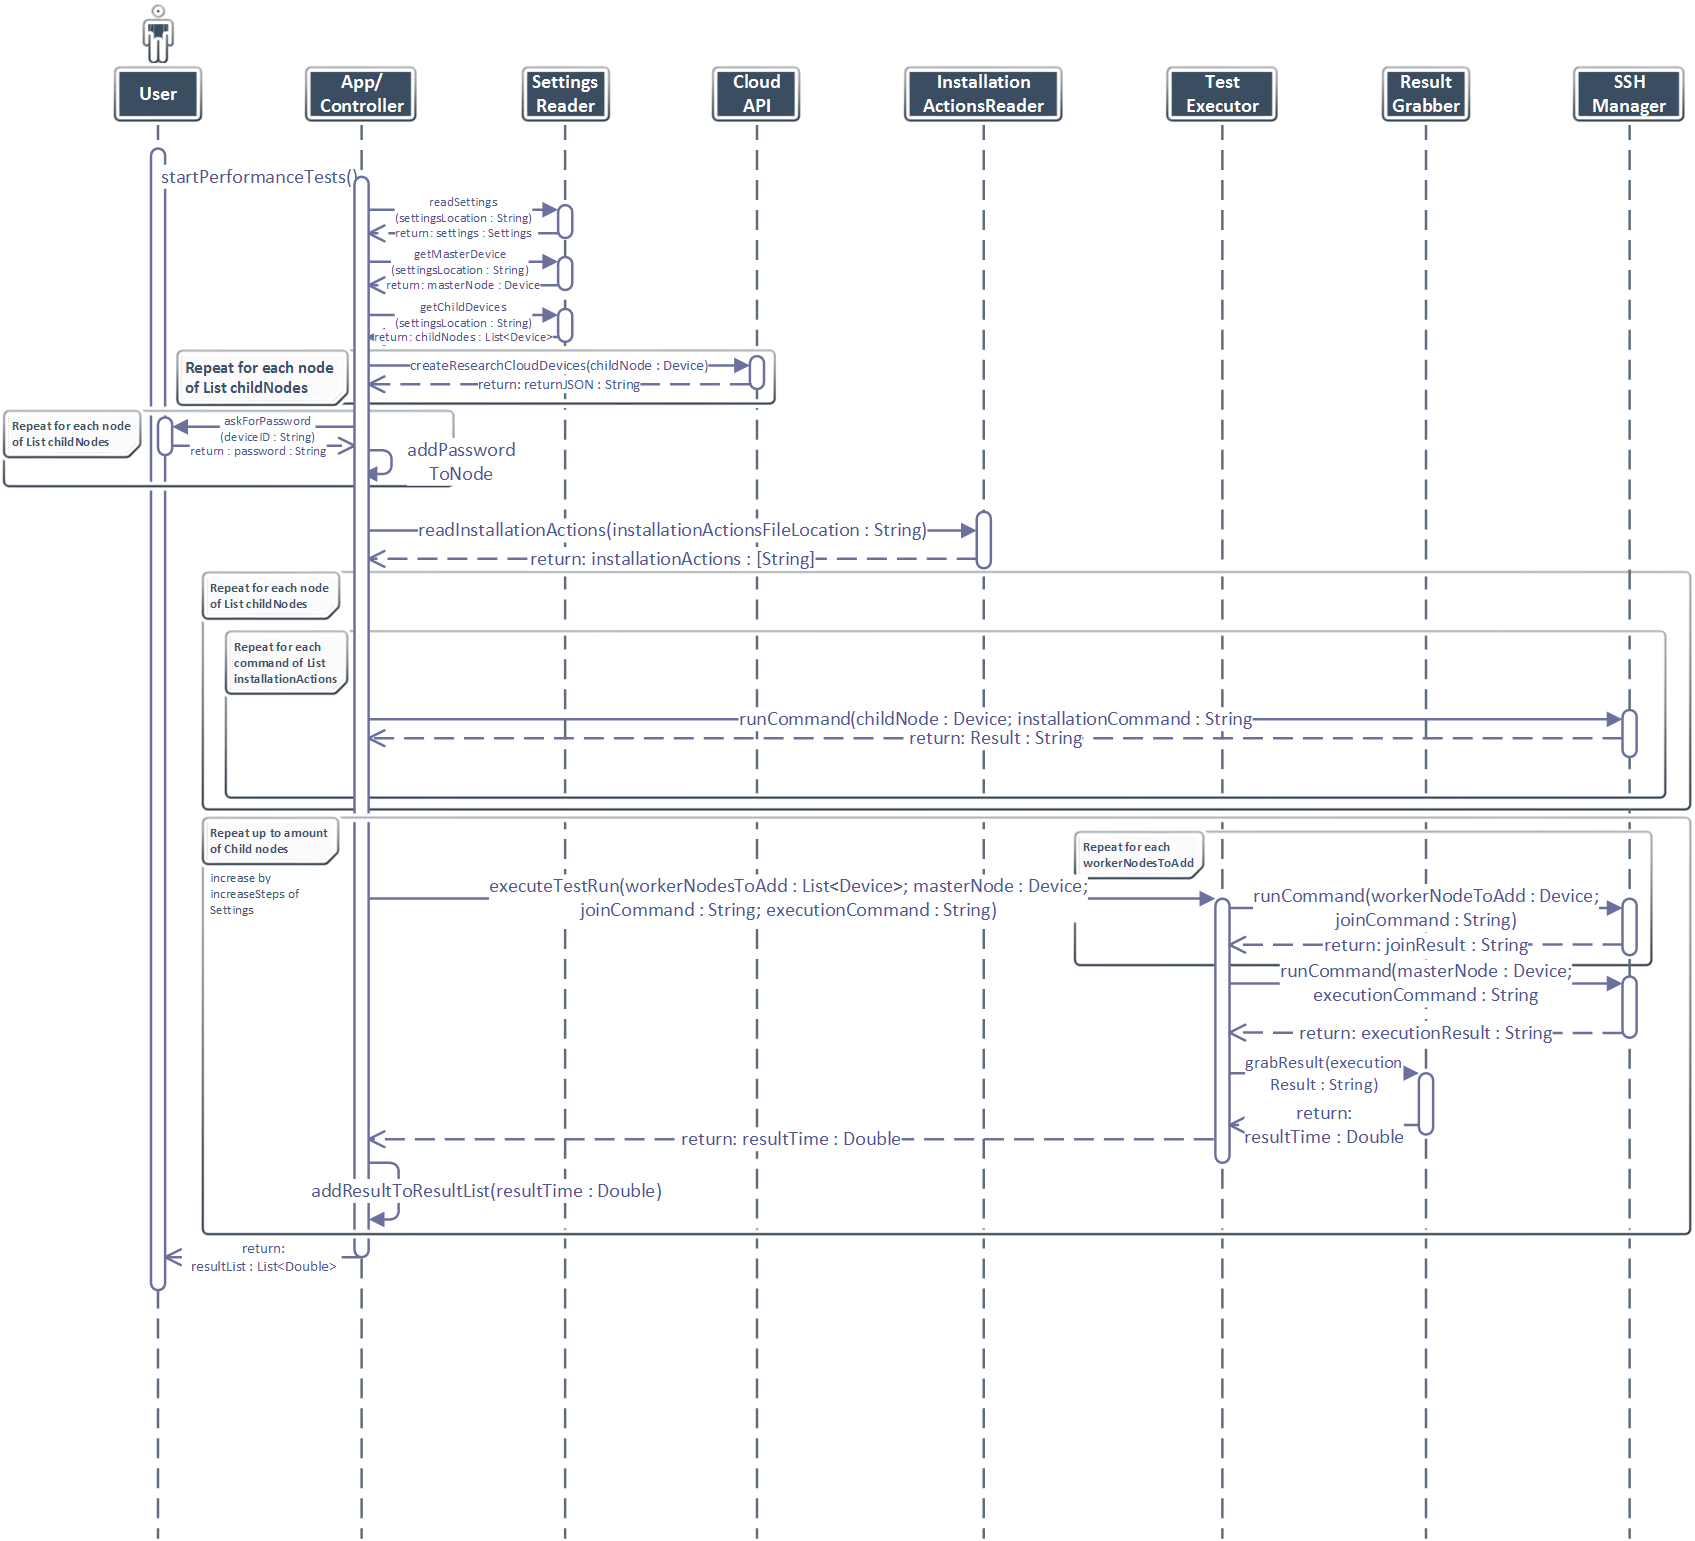
\includegraphics[width=\textheight/20*15]{images/testing_software_sequence_diagram.png}
}
\end{figure}